
\documentclass[12pt,a4paper,bibliography=totocnumbered,listof=totocnumbered]{scrartcl}
\usepackage[ngerman]{babel}
\usepackage[utf8]{inputenc}
\usepackage[T1]{fontenc} 
\usepackage{amsmath}
\usepackage{amsfonts}
\usepackage{amssymb}
\usepackage{graphicx}
\usepackage{fancyhdr}
\usepackage{tabularx}
\usepackage{geometry}
\usepackage{setspace}
\usepackage[right]{eurosym}
\usepackage[printonlyused,footnote]{acronym}
\usepackage{subfig}
\usepackage{floatflt}
\usepackage{float}
\usepackage[usenames,dvipsnames]{color}
\usepackage{colortbl}
\usepackage{paralist}
\usepackage{array}
\usepackage{titlesec}
\usepackage{parskip}
\usepackage[right]{eurosym}
% \usepackage{picins}
\usepackage[subfigure,titles]{tocloft}
\usepackage[pdfpagelabels=true]{hyperref}
\usepackage[svgnames,table,hyperref]{xcolor} % verschiedene Farbenauswahl
\usepackage{enumerate}
\usepackage{booktabs}
\usepackage{multirow}
\usepackage{url}
\usepackage{breakurl}
\usepackage[breaklinks]{hyperref}
\usepackage{placeins} % für FloatBarrier
\usepackage{enumitem}

\usepackage{wrapfig} % Wrap text around img
\usepackage{eurosym}

\def\UrlBreaks{\do\/\do-\do?\do_}

%\usepackage{minted}

%\usepackage{cite}
%\def\BibTeX{{\rm B\kern-.05em{\sc i\kern-.025em b}\kern-.08em
%    T\kern-.1667em\lower.7ex\hbox{E}\kern-.125emX}}
    
% generate uml diagram
%\usepackage{tikz} 
%\usetikzlibrary{arrows,shadows}
%\usepackage{pgf-umlsd}
\usepackage{framed}

\usepackage{epstopdf}
\epstopdfsetup{update}

\usepackage[font=normalsize,labelfont=bf,tableposition=top]{caption}

%\usepackage[babel, german=quotes, autostyle]{csquotes}
%\renewcommand{\blockquote}[1]{\textit{#1}}
%\renewcommand*{\mkblockquote}[4]{\textit{\enquote{#1}}#2#4#3}
%\renewcommand{\enqoute}[1]{\textit{#1}}

%\blockquote[{\cite[25]{ocit_o:protokoll}}] {text}
%\newcommand{\myblockquote}[2]{\blockquote[#1]{#2}}
\newenvironment{itquote}
{\begin{quote}\itshape}
{\end{quote}}
\newcommand{\itinquote}[1]{\textit{\glqq #1\grqq}}


\usepackage{listings}
\usepackage{verbatim}
\lstset{basicstyle=\footnotesize, captionpos=b, breaklines=true, showstringspaces=false, tabsize=2, frame=lines, numbers=left, numberstyle=\tiny, xleftmargin=2em, framexleftmargin=2em}
\makeatletter
\def\l@lstlisting#1#2{\@dottedtocline{1}{0em}{1em}{\hspace{1,5em} Lst. #1}{#2}}
\makeatother

%\usepackage[numbers,square]{natbib}  %neu
\usepackage[multiple,hang]{footmisc}

\renewcaptionname{ngerman}{\figurename}{Abb.}


\geometry{a4paper, top=27mm, left=31mm, right=21mm, bottom=35mm, headsep=10mm, footskip=12mm}
%\geometry{a4paper, top=27mm, left=30mm, right=20mm, bottom=35mm, headsep=10mm, footskip=12mm}

\hypersetup{unicode=false, pdftoolbar=true, pdfmenubar=true, pdffitwindow=false, pdfstartview={FitH},
	pdftitle={Studienarbeit: Web-Technologien},
	pdfauthor={Abwandner / Beham / Schmidt},
	pdfsubject={Ransomware},
	%pdfcreator={\LaTeX\ with package \flqq hyperref\frqq},
	pdfproducer={pdfTeX \the\pdftexversion.\pdftexrevision},
	pdfkeywords={},
	pdfnewwindow=true,
	colorlinks=false,linkcolor=blue,citecolor=blue,filecolor=magenta,urlcolor=blue}
\pdfinfo{/CreationDate (D:20160601000000)}

\definecolor{dunkelgrau}{rgb}{0.9,0.9,1.0}

\usepackage[
	backend=biber,
  %style=authoryear-icomp,
	style=authortitle-ibid,
	sortlocale=de_DE,
	natbib=true,
	url=true,
	doi=true,
	eprint=false
]{biblatex}

\addbibresource{library.bib}


\usepackage{afterpage}



\begin{document}

\titlespacing{\section}{0pt}{12pt plus 4pt minus 2pt}{-6pt plus 2pt minus 2pt}

% Kopf- und Fusszeile
\renewcommand{\sectionmark}[1]{\markright{#1}}
\renewcommand{\leftmark}{\rightmark}
\pagestyle{fancy}
\lhead{}
\chead{}
\rhead{\thesection\space\contentsname}
\lfoot{Ransomware}
\cfoot{}
\rfoot{\ \linebreak Seite \thepage}
\renewcommand{\headrulewidth}{0.4pt}
\renewcommand{\footrulewidth}{0.4pt}

% Vorspann
\renewcommand{\thesection}{\Roman{section}}
\renewcommand{\theHsection}{\Roman{section}}
\pagenumbering{Roman}

% -----------------------------------------------------------
% Deckblatt
% -----------------------------------------------------------
% -------------------------------------------------------------------
% Deckblatt
% -------------------------------------------------------------------
\thispagestyle{empty}
\begin{flushright}
	
\includegraphics[scale=0.3]{./hslogo}\\
\end{flushright}

\begin{minipage}[t]{0.78\textwidth}
	\Huge \textsf{\textbf{\textcolor{orange}{Studienarbeit: \\Web-Technologien}}}\\
	\Large \textsf{Studienrichtung Master Informatik}\\
\end{minipage}%
	\hfill
\begin{minipage}[t]{0.2\textwidth}
	{\textsf{\textcolor{orange}{Fakultät für\\ Informatik }}}
\end{minipage}%

\begin{flushleft}
	\vspace*{1cm}
	\huge
	\textsf{\textbf{\textcolor{orange}{Sebastian Abwandner \\ Paul Michael Beham \\ Pascal Schmidt }}\\
	Ransomware}\\
	\vspace*{0.5cm}
\end{flushleft}	
	\vfill
	\normalsize
	\newcolumntype{x}[1]{>{\raggedleft\arraybackslash\hspace{0pt}}p{#1}}
	
\begin{minipage}[t]{0.70\textwidth}
%	\vspace*{0.05cm}

	%\Large \textsf{
	\begin{large}
		{\sffamily
			\Large Betreuer: 
			\Large
			\begin{itemize}[label={}]
				\item Prof.~Dr.~Wolfgang Kowarschick
			\end{itemize}
		}
		\Large
		\vspace{0.5cm}
		{\sffamily
			Abgabe der Arbeit:
			\begin{itemize}[label={}]
				\item 07.01.2016
			\end{itemize}
		}
	\end{large}
\end{minipage}%
	\hfill
\begin{minipage}[t]{0.35\textwidth}
	\begin{small}
	\textsf{
	    \textcolor{red}{
		\noindent
		\mbox{}\\
		Hochschule Augsburg\\
		University of Applied Sciences\\
		An der Hochschule 1\\
		D-86161 Augsburg\\
		Telefon +49 821 5586-0\\
		Fax +49 821 5586-3222\\
		\href{http://www.hs-augsburg.de}{www.hs-augsburg.de}\\
		\href{mailto:info@hs-augsburg.de}{info@hs-augsburg.de}}\\
		\\
		Fakultät für Informatik\\
		Telefon: +49 821 5586-3450\\
		Fax: +49 821 5586-3499
		}
	\end{small}
\end{minipage}%



\pagebreak

\setcounter{page}{1}
\doublespacing
\titlespacing{\section}{0pt}{12pt plus 4pt minus 2pt}{2pt plus 2pt minus 2pt}
%\rhead{ERSTELLUNGSERKLÄRUNG}
\section*{Erstellungserklärung}
\vspace{2em}
% Hiermit versichere ich, Thomas Garron, dass ich die vorliegende Abschlussarbeit selbst- ständig und nur mit den angegebenen Hilfsmitteln verfasst habe. Ich erkläre ausdrücklich, dass ich sämtliche in der Arbeit verwendeten fremden Quellen, auch aus dem Internet, als solche kenntlich gemacht habe. Insbesondere bestätige ich, dass ich ausnahmslos sowohl bei wörtlich übernommenen Aussagen bzw. unverändert übernommenen Tabellen, Grafiken u. Ä. (Zitaten) als auch bei in eigenen Worten wiedergegebenen Aussagen bzw. von mir abgewandelten Tabellen, Grafiken u. Ä. anderer Autorinnen und Autoren (indirektes Zitieren) die Quelle angegeben habe.

Hiermit erklären wir, dass wir die vorgelegte Arbeit selbstständig verfasst, noch nicht anderweitig für Prüfungszwecke vorgelegt, keine anderen als die angegebenen Quellen oder Hilfsmittel verwendet sowie wörtliche und sinngemäße Zitate als solche gekennzeichnet haben.

\vspace{4em}
\begin{minipage}{\linewidth}
	\begin{tabular}{p{15em}p{15em}}
		Augsburg, den 22.06.2015 & 
		\underline{~~~~~~~~~~~~~~~~~~~~~~~~~~~~~~~~~~~~~~~~~~~}\\
		& 
		\centering Sebastian Abwandner
	\end{tabular}
\end{minipage}

\vspace{4em}
\begin{minipage}{\linewidth}
	\begin{tabular}{p{15em}p{15em}}
		Augsburg, den 22.06.2015 & 
		\underline{~~~~~~~~~~~~~~~~~~~~~~~~~~~~~~~~~~~~~~~~~~~}\\
		& 
		\centering Paul Michael Beham
	\end{tabular}
\end{minipage}

\vspace{4em}
\begin{minipage}{\linewidth}
	\begin{tabular}{p{15em}p{15em}}
		Augsburg, den 22.06.2015 & 
		\underline{~~~~~~~~~~~~~~~~~~~~~~~~~~~~~~~~~~~~~~~~~~~}\\
		& 
		\centering Pascal Schmid
	\end{tabular}
\end{minipage}
%\begin{minipage}{\linewidth} 
%	\begin{tabular}{p{15em}p{15em}}
%		..................................... & 
%		....................................................... \\
%		Datum & 
%		\centering (Unterschrift)
%	\end{tabular}
%\end{minipage}

\pagebreak % TODO

%\include{chapters/nda}

% -----------------------------------------------------------
% Abstract
% -------------------------------------------------------------
%\include{chapters/kurzfassung}


% -----------------------------------------------------------
% Verzeichnisse
% -----------------------------------------------------------
%% TODO Typ vor Nummer
%\renewcommand{\cfttabpresnum}{Tab. }
%\renewcommand{\cftfigpresnum}{Abb. }
%\settowidth{\cfttabnumwidth}{Abb. 10\quad}
%\settowidth{\cftfignumwidth}{Abb. 10\quad}
%\setlength{\cftsecnumwidth}{2.5em}% Set length of number width in ToC for \subsection
%\titlespacing{\section}{0pt}{12pt plus 4pt minus 2pt}{2pt plus 2pt minus 2pt}
%\singlespacing
\rhead{INHALTSVERZEICHNIS}
%\renewcommand{\contentsname}{III Inhaltsverzeichnis}
%\phantomsection
%\addcontentsline{toc}{section}{\texorpdfstring{III \ \  \hspace{0.35em}Inhaltsverzeichnis}{Inhaltsverzeichnis}}
%\addtocounter{section}{1}
\onehalfspacing
\tableofcontents % Write out the Table of Contents (Inhaltsverzeichnis)
\pagebreak
\doublespacing
% -----------------------------------------------------------
% Inhalt
% -----------------------------------------------------------
% Abstände Überschrift
\titlespacing{\section}{0pt}{12pt plus 4pt minus 2pt}{-6pt plus 2pt minus 2pt}
\titlespacing{\subsection}{0pt}{12pt plus 4pt minus 2pt}{-6pt plus 2pt minus 2pt}
\titlespacing{\subsubsection}{0pt}{12pt plus 4pt minus 2pt}{-6pt plus 2pt minus 2pt}

% Kopfzeile
\renewcommand{\sectionmark}[1]{\markright{#1}}
\renewcommand{\subsectionmark}[1]{}
\renewcommand{\subsubsectionmark}[1]{}
\lhead{Kapitel \thesection}
\rhead{\rightmark}

\doublespacing
\renewcommand{\thesection}{\arabic{section}}
\renewcommand{\theHsection}{\arabic{section}}
\setcounter{section}{0}
\pagenumbering{arabic}
\setcounter{page}{1}

% -----------------------------------------------------------
% Einzelne Kapitel:
% Einleitung - zum Thema führen, warum wichtig, welche Gesichtspunkte, Aktuelles
% Related Work - Literatur, Papers, wiss. Lücke, Forschungsfrage
% Hintergrund - Algorithmen, Funktionsweisen, auch: Festplattenfunktion 10-15 Seiten
% Evaluation - Use Cases, Tools, Funktionalitäten, Bewertung
% Conclusion - Future Work
% -----------------------------------------------------------

%\include{chapters/chapter_1_einleitung}
%\include{chapters/chapter_2_related}
%\include{chapters/chapter_3_hintergrund}
%\include{chapters/chapter_4_evaluation}
%\include{chapters/chapter_5_conclusion}


\begin{abstract}
Wir beschreiben den in den letzten Jahren bekannt gewordenen Malware-Typ der Ransomware. Hierbei wird auf die geschichtliche Entwicklung und die Gründe für die späte Entstehung dieser Malware eingegangen. Für das Verständnis ist es zudem wichtig eine kurze Zusammenfassung über Kryptographie und anonyme Bezahlmöglichkeiten zu geben. Abschließend sollen Möglichkeiten und Grenzen von Gegenmaßnahmen erläutert werden.
\end{abstract}

\section{Einleitung}
\label{sec:einleitung}
	In den letzten Jahren haben sich die bekannt gewordenen Fälle von Ransomware vervielfacht. Waren früher noch irreführende Apps der Hauptanteil der Malware, wurde 2012 mit den sogenannten Lockern erstmals Malware entdeckt, die großflächig die betroffenen Anwender zur Bezahlung einer Lösegeldsumme veranlasst hat. In den Jahren 2014 und 2015 wurden diese eher harmlosen Varianten, die nur die Benutzung des Geräts blockiert haben, durch die Cryptoransomware abgelöst. Diese verschlüsselt die Dateien des Benutzers und fordert zum Wiedererhalt eine Lösegeldsumme, die nicht-verfolgbar bezahlt werden soll.

	\begin{figure}[h!]
		\centering
		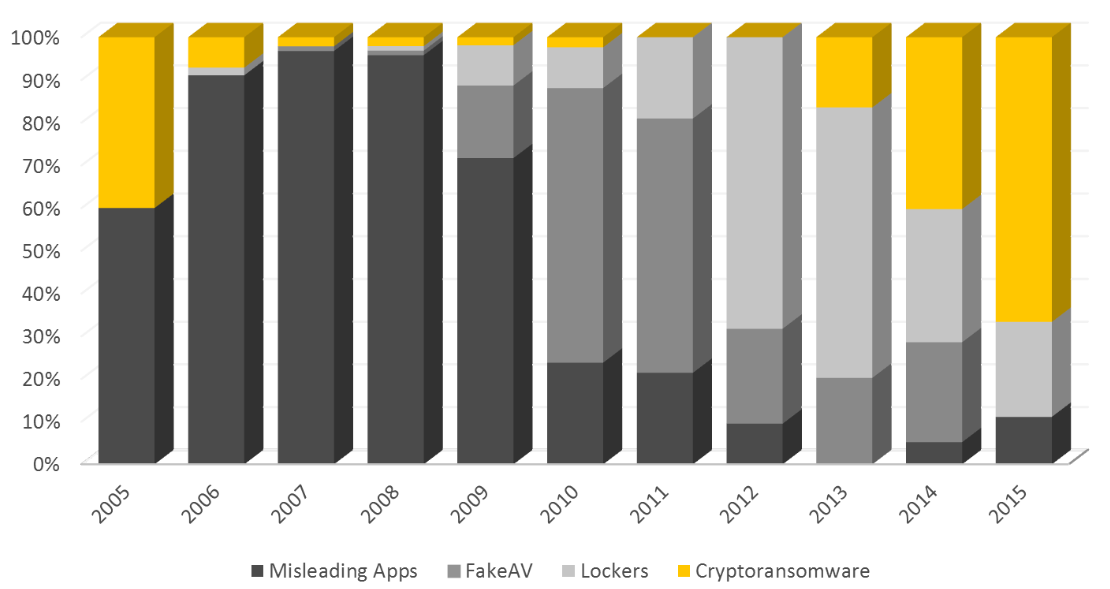
\includegraphics[width=\linewidth]{img/ransom-evolution.png}
		\caption{Evolution Malware \\ Quelle: \cite{aids:sdf}}
		\label{fig:ransom-evo}
	\end{figure}

\section{Definition Schadsoftware}
\label{sec:definition}
		Aufgrund der teilweise überschneidenen Funktionen im Bereich der Malware ist es schwierig eine allgemeingültige Definition für diese zu finden, im Rahmen dieser Arbeit soll sich jedoch an die Definitionen des Microsoft Protection Centers \cite{malware_pc} gehalten werden.

		\begin{itemize}
			\item \textbf{Bot:} Ein kleines, versteckes Programm auf dem Rechner des Benutzers, oftmals vom Angreifer kontrolliert. Mehrere Bots, die über das Netzwerk verbunden sind, nennt man ein Netzwerk.
			\item \textbf{Botnetz:} Mehrere Kopien des­sel­ben Bots sind auf mehreren Rechnern installiert und werden von einem böswilligen Hacker kontrolliert. Mehrere Bots auf einer großen Anzahl infizierter Rechner nennt man Botnetz.
			\item \textbf{Malware:}	Kurzform für ``malicious software''. Überbegriff für Software, die ungewollte Aktivitäten auf einem Rechner durchführt, wie etwa Daten stehlen, Dateien verschlüsseln oder Spam verschickt.
			\item \textbf{Ransomware:} Eine Art Malware, die den Benutzer daran hindert das Gerät zu benutzen oder die Dateien verschlüsselt. Der Benutzer wird darüber informiert, dass er Geld bezahlen, eine Befragung durchführen oder eine sonstige Aktion durchführen muss, bevor er die Kontrolle wiedererlangt.
			\item \textbf{Trojaner:} Nach dem Trojanischen Pferd aus der Sage benannt, verhält sich diese Art von Malware unauffällig, um nicht entdeckt zu werden. Im Gegensatz zu Würmern oder Viren verbreitet sich ein Trojaner nicht von selbst weiter, sondern täuscht den Benutzer, um von diesem heruntergeladen oder installiert zu werden.
			\item \textbf{Virus:} Malware, die sich selbst weiterverbreitet, indem es reguläre Programme befällt und sich auf andere Systeme und Netzwerke weiterverbreitet.
			\item \textbf{Wurm:} Ein Wurm unterscheidet sich vom Virus dadurch, dass er mithilfe eines Trägers verbreitet wird. Dies kann etwa durch E-Mails, Instant Messaging, File-Sharing, Netzwerklaufwerke, Wechsellaufwerke und Ähnliches geschehen.
		\end{itemize}

\section{Geschichte der Ransomware}
\label{sec:geschichte}
	\subsection{AIDS}
		Gemeinhin gilt der \textsc{AIDS Information Trojaner} als erste Ransomware im heutigen Sinne, da dieser nicht nur den Computer des Opfers unbrauchbar machte, sondern
		parallel dazu eine "`Reparatur"' gegen Bezahlung anbot. \\
		Getarnt als Anwendung zur Abschätzung des Risikos einer HIV-Infektion und als aktuelle Informationsdatenbank nutzte der 1989 entstandene Virus die damalige
		Unsicherheiten bezüglich einer HIV-Infektion aus, um so eine Installation und auch eine größere Verbreitung zu erreichen.
	\begin{figure}[h!]
		\centering
		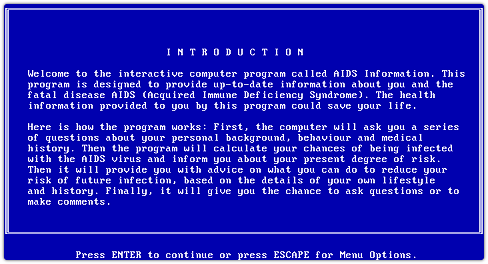
\includegraphics[width=\linewidth]{img/aids1.png}
		\caption{Lizenzvereinbarung AIDS \\ Quelle: \cite{aids:sophos}}
		\label{fig:lizenz_aids}
	\end{figure}

		Nach der Installation wurde mittels eines Zählers in der Autostart-Datei des Systems ermittelt, wie oft der Computer gestartet worden ist. War der 90. Start
		erreicht, verschlüsselte der Virus die Namen von vordefinierten Dateien und Verzeichnissen, nicht aber deren Inhalt. Dies betraf auch wichtige Systemprogramme, die
		ein Kommando-orientiertes Betriebssystem wie MS-DOS erst benutzbar machen. \\
		Zeitgleich wurde dem Opfer eine Nachricht gezeigt, mit den genauen Anweisungen, wie die vorgebliche Nutzungsgebühr an den Hersteller zu bezahlen sei.
		Scheinbar legitimiert wird dieses Vorgehen mit den Lizenzvereinbarungen, die während der Installation vom Benutzer akzeptiert wurden.

		Eine Analyse des Virus zeigte, dass vor allem die Verwendung einer symmetrischen Verschlüsselung (siehe Kapitel~\ref{sec:sym_verschl}).
		Da hierfür die Schlüssel für die Ver- und Entschlüsselung gleich sind und prinzipbedingt im Virus selbst hinterlegt sein müssen, bot sich hier ein Angriffspunkt, um die
		Verschlüsselung auch ohne Zahlung der geforderten Geldsumme umzukehren. Erleichternd kommt hier dazu, dass die Schlüssel hart-codiert sind, und alle Infektionen
		den gleichen Schlüssel verwenden. \\
		So ist es nicht verwunderlich, dass sich bald Entschlüsselungswerkzeuge verbreiteten und damit die Wirkung des Virus außer Kraft setzten. \\
		Eine Untersuchung durch Adam Young und Moti Yung, schlug hier die Verwendung von asymmetrischer Verschlüsselung (siehe Kapitel~\ref{sec:asym_verschl}) vor, um einen
		Vorteil über das Opfer zu erhalten. \footcite{aids:young}

		Die Autoren heutiger Ransomware haben sich diesen Vorschlag zu Herzen genommen, sodass eine asymmetrische Verschlüsselung heute fast ausnahmslos in Ransomware
		verwendet wird. Auch entscheidende Konzepte von AIDSinfo werden immer noch benutzt, sei des einen vorgeblichen Nutzen des Programms anzubieten oder auch nicht
		direkt nach der Infektion aktiv zu werden, sondern noch einige Zeit abzuwarten.

\section{Überblick über aktuelle Ransomware}
\label{sec:overview}
		Alle hier beschriebenen Ransomware sind innerhalb des letzten Jahres erschienen und beschreiben somit den zum Schreiben des vorliegenden Papers aktuellen Stand der Technik.

		\subsection{TeslaCrypt}
			TeslaCrypt war der erste der modernen Ransomware, der von den Medien aufgegriffen wurde und somit der Öffentlichkeit bekannt gemacht wurde. Ende 2015\cite{tesla:entdeckt} wurde dieser entdeckt, jedoch wurde bereits kurze Zeit später ein Tool veröffentlicht\cite{tesla:geknackt}, mit dem betroffene Anwender ihre Daten retten konnten.
			Version 3 der Ransomware wurde von den Angreifern grundlegend verändert. So wurde der Algorithmus zum Schlüsselaustausch erneuert, was es vorerst unmöglich gemacht hat, den privaten Schlüssel der Ransomware aus den verschlüsselten Dateien herzustellen\cite{tesla:version3}\cite{tesla:version3_2}.
			Die letzte Version 4 kann zudem Dateien größer als 4 GB verschlüsseln\cite{tesla:version4}.....
		\subsection{Petya}
		\subsection{Locky}
		\subsection{KeRanger}


\section{Faktoren von Ransomware}
	Ökonomie / Psychologie / Social-Engineering

\section{Überblick Verschlüsselung}
Dieses Kapitel soll eine kurze Einführung über Verschlüsselungen geben, allerdings wird hier im Rahmen der Lesbarkeit auf mathematische Exaktheit verzichtet. Ebenso werden
die einzelnen Punkte nur insoweit erklärt und beschrieben, wie für ein Verständnis über deren Anwendung in Rahmen von Ransomware notwendig ist.

Für genauere Betrachtungen sei die einschlägige Fachliteratur hierüber empfohlen. % Beispiele
\subsection{Symmetrische Verschlüsselung}
\label{sec:sym_verschl}

Die symmetrische Verschlüsselung folgt dem Konzept, das sowohl für die Ver- als auch die Entschlüsselung jeweils die gleichen Schlüssel verwendet werden.
\afterpage{
\begin{figure}[h!]
	\centering
	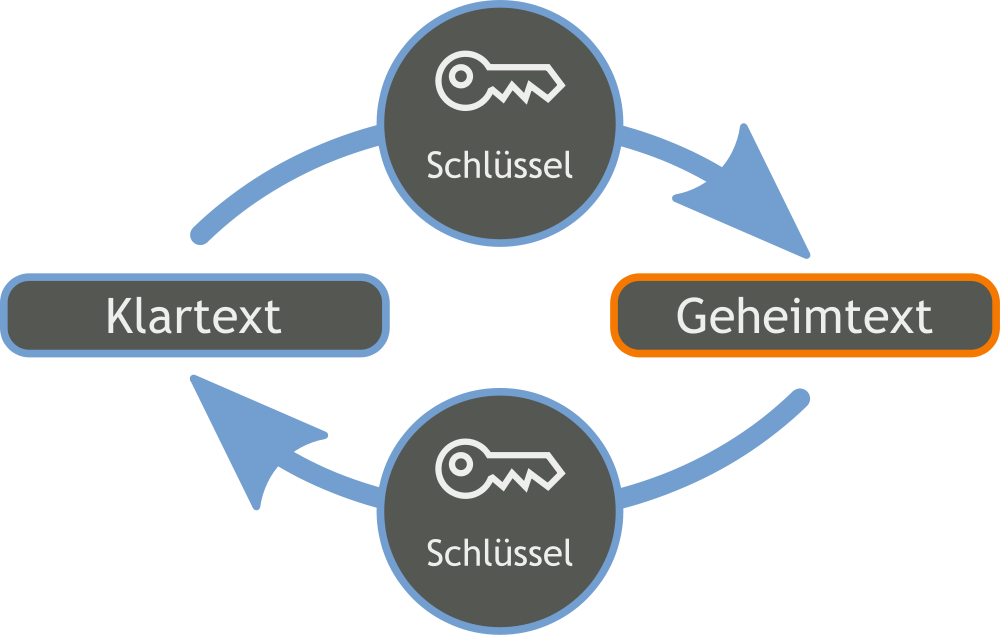
\includegraphics[width=\linewidth]{img/SymKrypto.png}
	\caption{Symmetrische Verschlüsselung mit identischen Schlüsseln}
	\label{fig:sym_verschl}
	\end{figure}
	\footnotetext{Quelle: Bananenfalter (Public Domain) \\ \url{https://commons.wikimedia.org/wiki/File:Orange_blue_symmetric_cryptography_de.svg}}
}
Es gibt eine Reihe an unterschiedlichsten Algorithmen und Verfahren für symmetrische Verschlüsselung, allerdings hat sich mit \textsc{AES} ein Verfahren als de-facto Standard für verschiedenste Anwendungsbereiche etabliert.

AES ist hierbei eine Abkürzung für Advanced Encryption Standard und wird meist synonym für den Rijndael-Algorithmus verwendet. Dieses Verfahren ist heute so verbreitet, dass beispielsweise in modernen Prozessoren direkt als Maschinenbefehl zur Verfügung steht und somit deutlich größere Datenraten verarbeiten kann. \\
Benchmarks zeigen hier beispielshaft einen 6-fachen Speedup mit einer Datenrate von ca. 1.35 GB/s mit CPU-Unterstützung verglichen mit 212 MB/s ohne
CPU-Unterstützung.\footcite{aes:benchmark}

Vor allem durch die Hardware-Unterstützung ist es moderner Ransomware möglich, die CPU-Last während der Verschlüsselung derart in Grenzen zu halten, dass der Nutzer keine spürbare Langsamkeit des Systems bemerkt.


\subsection{Asymmetrische Verschlüsselung}
\label{sec:asym_verschl}

\afterpage{
\begin{figure}[h!]
	\centering
	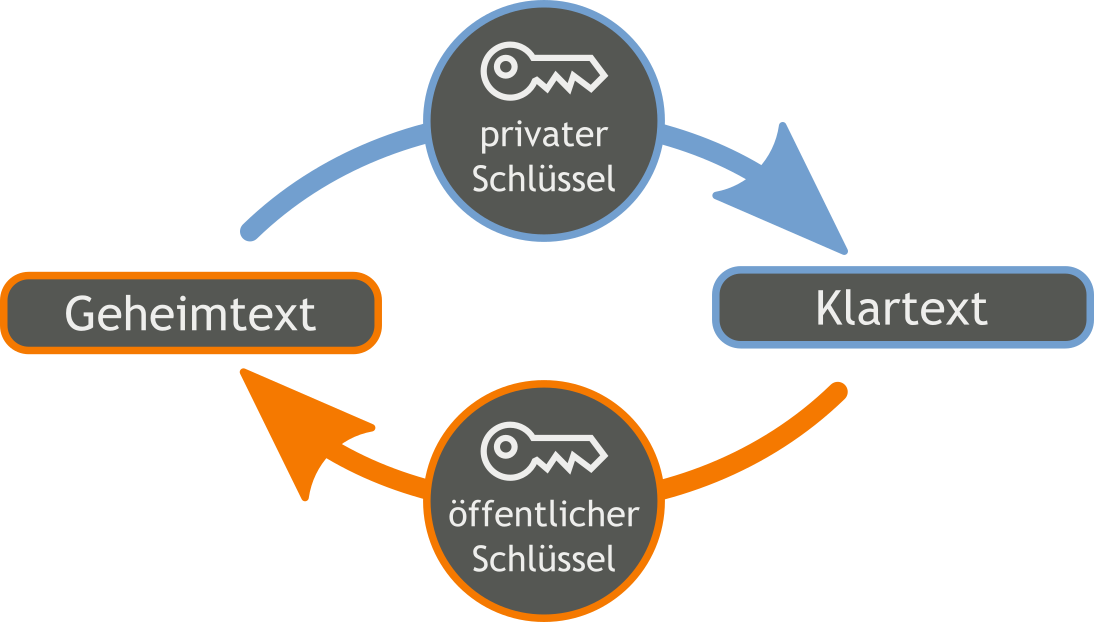
\includegraphics[width=\linewidth]{img/AsymKrypto.png}
	\caption{Asymmetrische Verschlüsselung}
	\label{fig:asym_verschl}
	\end{figure}
	\footnotetext{Quelle: Bananenfalter (Public Domain) \\ \url{https://commons.wikimedia.org/wiki/File:Orange_blue_symmetric_cryptography_de.svg}} %TODO: Url
}

Asymmetrische Verschlüsselung basiert auf zwei Schlüsseln, einen öffentlichen und einen privaten. Diese Schlüssel gehören mathematisch zusammen und werden für unterschiedliche Zwecke verwendet.
Soll ein Klartext verschlüsselt werden, so wird hierfür der öffentliche Schlüssel des Empfängers verwendet. Die Entschlüsselung muss dann mit dem zugehörigen privaten Schlüssel erfolgen, eine Entschlüsselung mit dem öffentlichen Schlüssel ist nicht mehr möglich.

Auf Grund der Komplexität der Berechnungen ist das Verfahren langsam und auch nur schwer in Hardware abzubilden. Deshalb wird es nur für verhältnismäßig kurze Klartexte verwendet (< 1 KB), auch da die maximale Länge des Klartexts von der Länge des verwendeten Schlüssels abhängt. %TODO: Nachweis


Der große Vorteil von asymmetrischer Verschlüsselung liegt im sicheren Schlüsselaustausch, der nicht auf einen bereits gesicherten Kanal angewiesen ist, sondern auch über ein unsicheres Medium, beispielsweise über das Internet erfolgen kann, ohne dass es für einen Angreifer möglich ist die beteiligten Schlüssel zu belauschen oder zu berechnen. %TODO: MitM




\subsection{Hybride Verschlüsselung}
\label{sec:hybride_verschl}

Hybride Verschlüsselung kombiniert alle Vorteile von symmetrischer Verschlüsselung (Geschwindigkeit, Einfachheit) mit allen Vorteilen von asymmetrischer Verschlüsselung (Schlüsseltausch, Sicherheit).
Hierfür werden zufällige Schlüssel erzeugt, meist lange Zufallszahlen, die für die symmetrische Verschlüsselung verwendet werden. Diese Schlüssel werden Sitzungsschlüssel genannt und werden in der Regel nur einmalig verwendet (ein sog. One-Time-Pad). Nach der Verwendung werden die Sitzungsschlüssel asymmetrisch verschlüsselt und mit den codierten Daten zusammen übertragen.

Auf diese Weise lassen sich auch große Mengen an Daten effizient mittels asymmetrischer Kryptographie übertragen.




\section{Überblick Anonyme Zahlungen}
Eine weitere Komponente warum heutige Ransomware so erfolgreich ist, stellt die Möglichkeit einer anonymen Bezahlung dar, vor allem in Hinsicht auf die Anonymität des Zahlungsempfängers. Hier stehen dem Angreifer verschiedene Zahlungsverfahren zur Auswahl, von eher traditioneller Überweisung bis hin zu Bitcoins.

\subsection{Ukash}
\subsection{Paysafecard}
\subsection{Western Union}
\subsection{Bitcoin}

\section{Überblick Tor-Netzwerk}
	Tor / Aufbau / Hidden Services / Anonymität

\section{Genereller Ablauf}
 CC Server / Verschlüsselung / Zahlung

\section{Weitere Beobachtungen}
Ransomware as a service

\section{Gegenmaßnahmen}

Backups / Heuristiken / Backups / Nutzerschulung / Backups /

\section{Schluss}

%\appendix
%\include{chapters/appendix} % TODO: Testplan

% -----------------------------------------------------------
% einzelne Verzeichnisse
% -----------------------------------------------------------

%\renewcommand{\thesection}{\Roman{section}}
%\renewcommand{\theHsection}{\Roman{section}}
%%\pagenumbering{Roman}
%\renewcommand{\cfttabpresnum}{Tab. }
%\renewcommand{\cftfigpresnum}{Abb. }
%%\settowidth{\cfttabnumwidth}{Abb. 10\quad}
%%\settowidth{\cftfignumwidth}{Abb. 10\quad}
%\setcounter{section}{3}
%
%\rhead{VERZEICHNISSE}
%\titlespacing{\section}{0pt}{12pt plus 4pt minus 2pt}{2pt plus 2pt minus 2pt}
%\renewcommand*\listfigurename{Abbildungsverzeichnis \vspace{1em}}

%\listoffigures
%\listoftables

%\addtocontents{lof}{\vspace{-0.5em}}
% \renewcommand{\vspace}[2]{}% Gobble 2 arguments after \vspace
\pagebreak

%\listoftables % Write out the List of Tables (Tabellenverzeichnis)
%\pagebreak
%\renewcommand{\lstlistlistingname}{Listing-Verzeichnis}
%{\labelsep2cm\lstlistoflistings}
%\pagebreak

% -------------------------------------------------------------
% Abkürzungen
% -----------------------------------------------------------
%\include{chapters/abkuerzungsverzeichnis}


% -------------------------------------------------------------
% Literatur
% -------------------------------------------------------------
\renewcommand\refname{Literaturverzeichnis}
%\bibliographystyle{abstract}

% Weitere Möglichkeiten für Quellenangaben
%\bibliographystyle{plaindin}
%%%\bibliographystyle{plainurl}
%\bibliographystyle{alphadin}
%\bibliographystyle{natdin}

\nocite{*}
\printbibliography

Alle Links wurden zuletzt \today ~besucht.
\pagebreak

% -----------------------------------------------------------
% Anhang
% -----------------------------------------------------------
%\pagenumbering{Roman}
%\setcounter{page}{1}

%\lhead{Anhang \thesection}

%\begin{appendix}
%\section*{Anhang}
%\phantomsection
%\addcontentsline{toc}{section}{Anhang}
%\addtocontents{toc}{\vspace{-0.5em}}

%\section{view.dtd}\label{anhang:dtd}
%\verbatiminput{document/view_v1.dtd} % Anfügen von Text-Dateien
%\pagebreak

%\section{pom.xml}\label{anhang:pom}
%\verbatiminput{document/pom.xml}


%\subsection*{Screenshot}
%\label{app:screenshot}
%Unterkategorie, die nicht im Inhaltsverzeichnis auftaucht.

%\end{appendix}



\end{document}